\documentclass[10pt,twocolumn]{article}

% arXiv preprint format
\usepackage[utf8]{inputenc}
\usepackage[T1]{fontenc}
\usepackage{times}
\usepackage[margin=1in]{geometry}
\usepackage{graphicx}
\usepackage{amsmath,amssymb}
\usepackage{booktabs}
\usepackage{hyperref}
\usepackage{xcolor}
\usepackage{multirow}
\usepackage{array}

% Graphics path (figures in same directory as .tex)
\graphicspath{{./}}

\title{Communication-Efficient Distributed Vector Memory:\\ Investigating Adaptive Routing Across Partitioned Semantic Memories}

\author{
  Agostina Silva
}

\date{}

\begin{document}

\maketitle

\begin{abstract}
Distributed vector databases partition embeddings across multiple servers to achieve scalability, but querying all partitions (broadcasting) incurs communication costs that grow linearly with the number of partitions. We investigate whether adaptive inter-partition communication can achieve retrieval performance comparable to a centralized index while requiring significantly less communication. We propose four routing strategies---Confidence Threshold, Top-N Neighbors, Progressive Expansion, and Budgeted Communication---that dynamically determine which partitions to query based on local confidence estimation. Using DBpedia 14 (100K documents across 14 semantic classes), all-MiniLM-L6-v2 embeddings, and TurboVec (TurboQuant) for 4-bit quantized indexing, we evaluate these strategies across 2, 4, 8, and 16 partitions. Our results show that adaptive routing achieves 100\% of global recall (0.939) while contacting only 58\% of partitions at K=16, representing a 42\% reduction in communication. We further demonstrate that semantic partitioning (KMeans) outperforms random partitioning by 8--12\%, validating the importance of coherent semantic structure. These findings suggest that intelligent routing can significantly reduce communication costs in distributed vector search systems without sacrificing retrieval quality.
\end{abstract}

\section{Introduction}

Modern vector databases (Milvus, Weaviate, Qdrant) achieve scalability by partitioning embeddings across multiple servers~\cite{pyramid,fedvs}. However, querying all partitions---a broadcast---incurs communication costs that grow linearly with the number of partitions $K$, creating a fundamental tension between retrieval quality and system efficiency.

Consider a distributed semantic memory with $K$ independent partitions, each containing a subset of the document embeddings. A broadcast query contacts all $K$ partitions, achieving maximum recall but requiring $O(K)$ communication. Conversely, querying only the nearest partition reduces communication to $O(1)$ but risks missing relevant documents stored in other partitions.

\textbf{Open problem:} Can intelligent routing find a middle ground---achieving recall comparable to broadcasting while requiring sub-linear communication?

We propose four adaptive routing strategies that dynamically determine which partitions to contact based on confidence estimation:

\begin{enumerate}
    \item \textbf{Confidence Threshold}: Expand search when local confidence falls below a threshold
    \item \textbf{Top-N Neighbors}: Always query the $N$ closest partitions
    \item \textbf{Progressive Expansion}: Expand until a confidence target is met
    \item \textbf{Budgeted Communication}: Enforce a hard limit on partitions contacted
\end{enumerate}

\textbf{Contributions:}
\begin{itemize}
    \item A confidence estimation formula that penalizes low partition coverage, forcing expansion even when local scores appear confident
    \item Four routing strategies that reduce communication by 42--75\% while retaining 97--100\% of global recall
    \item Empirical validation that semantic partitioning (KMeans) outperforms random partitioning by 8--12\%, demonstrating the importance of coherent cluster structure
    \item Analysis of the communication-quality tradeoff across multiple partition counts
\end{itemize}

\section{Related Work}

\subsection{Distributed Vector Search}

Distributed vector search systems partition embeddings across multiple nodes to achieve horizontal scalability. FedVS~\cite{fedvs} proposes a federated approach to vector search with communication-efficient protocols. Pyramid~\cite{pyramid} provides a framework for distributed similarity search with hierarchical partitioning. d-HNSW~\cite{dhnsw} extends the Hierarchical Navigable Small World algorithm to distributed settings, maintaining graph connectivity across partitions.

\subsection{Adaptive Routing}

Routing in distributed systems has been studied in various contexts. ShardMemo~\cite{shardmemo} introduces shard-based memory with configurable probe budgets to limit communication. HyphaeDB~\cite{hyphaedb} employs graph-based neighbor routing inspired by biological networks. RAGRoute~\cite{ragroute} proposes routing strategies specifically designed for Retrieval-Augmented Generation systems.

\subsection{Quantization for Vector Databases}

Vector quantization reduces memory footprint and computational cost. TurboQuant~\cite{turboquant}, introduced at ICLR 2026, achieves data-oblivious quantization with near-optimal distortion without requiring a training phase. This makes it particularly suitable for dynamic systems where vectors are added incrementally.

\subsection{Hierarchical Index Structures}

HNSW~\cite{hnsw} provides efficient approximate nearest neighbor search through hierarchical graph navigation. Pyramid~\cite{pyramid} proposes pyramid-based partitioning for distributed search, assigning queries to only relevant sub-datasets for high throughput.

\section{Methodology}

\subsection{System Model}

Consider a distributed vector memory with $K$ independent partitions $\{P_1, P_2, \ldots, P_K\}$, each containing a subset of $N$ document embeddings $\{\mathbf{e}_1, \mathbf{e}_2, \ldots, \mathbf{e}_N\} \subset \mathbb{R}^d$. Each partition maintains its own vector index (TurboVec) and centroid $\mathbf{c}_k$ representing the mean embedding of its documents.

Given a query embedding $\mathbf{q}$, the system must retrieve the top-$k$ most similar documents across all partitions while minimizing the number of partitions contacted.

\subsection{Confidence Estimation}

We propose a confidence estimation formula that combines score-based confidence with partition coverage:

\begin{equation}
    \text{confidence} = \sigma(\text{gap}) \times \frac{n_{\text{contacted}}}{n_{\text{total}}}
\end{equation}

where:
\begin{itemize}
    \item $\sigma(x) = \frac{1}{1 + e^{-5x}}$ is a sigmoid function
    \item $\text{gap} = s_1 - \frac{1}{k-1}\sum_{i=2}^{k} s_i$ is the difference between the top score and mean of remaining scores
    \item $n_{\text{contacted}}$ is the number of partitions queried so far
    \item $n_{\text{total}}$ is the total number of partitions
\end{itemize}

\textbf{Key insight:} The coverage term $\frac{n_{\text{contacted}}}{n_{\text{total}}}$ penalizes low partition coverage. Even if the top score appears confident (high gap), the overall confidence remains low when few partitions have been contacted. This forces the routing algorithm to expand its search, preventing premature termination.

\subsection{Routing Strategies}

\subsubsection{Confidence Threshold}
Search the nearest partition first. If confidence $< \theta$, progressively query remaining partitions sorted by centroid distance until confidence $\geq \theta$.

\subsubsection{Top-N Neighbors}
Always query the $N$ nearest partitions by centroid distance, regardless of confidence.

\subsubsection{Progressive Expansion}
Start with the nearest partition. Progressively add partitions until confidence reaches target $\theta$.

\subsubsection{Budgeted Communication}
Query at most $M$ partitions, where $M < K$.

\section{Experimental Setup}

\subsection{Dataset}

We use DBpedia 14~\cite{zhang2015character}, a standard text classification benchmark consisting of 630K documents across 14 non-overlapping semantic classes: Company, EducationalInstitution, Artist, Athlete, OfficeHolder, MeanOfTransportation, Building, NaturalPlace, Village, Animal, Plant, Album, Film, and WrittenWork. We subsample 100K documents for computational efficiency while maintaining class balance (45K documents per class in the full dataset).

\subsection{Embedding Model}

We use all-MiniLM-L6-v2~\cite{reimers2019sentence}, a 384-dimensional sentence transformer trained on 1B+ sentence pairs. Embeddings are L2-normalized for cosine similarity computation.

\subsection{Partitioning}

We employ KMeans clustering with $K \in \{2, 4, 8, 16\}$ to create semantically coherent partitions. As a baseline, we also evaluate random partitioning (uniform random assignment to partitions).

\subsection{Vector Index}

We use TurboVec (TurboQuant)~\cite{turboquant} with 4-bit quantization (16 quantization levels), achieving 8$\times$ compression compared to float32 representations. Each partition maintains an independent TurboVec index.

\subsection{Evaluation Metrics}

\begin{itemize}
    \item \textbf{Recall@10}: Fraction of ground truth top-10 results retrieved
    \item \textbf{MRR}: Mean Reciprocal Rank of first relevant result
    \item \textbf{NDCG@10}: Normalized Discounted Cumulative Gain at 10
    \item \textbf{Communication Cost}: Average number of partitions contacted per query
    \item \textbf{Communication Reduction}: $1 - \frac{n_{\text{contacted}}}{K}$ (percentage of partitions not contacted)
\end{itemize}

Ground truth is computed via exact cosine similarity search over all embeddings.

\section{Results}

\subsection{Main Results}

Table~\ref{tab:main_results} presents the comprehensive results across all partition counts and strategies.

\begin{table*}[t]
\centering
\caption{Comprehensive results across all partition counts and strategies. Recall@10, MRR, and NDCG@10 are averaged over 100 queries.}
\label{tab:main_results}
\small
\resizebox{\textwidth}{!}{%
\begin{tabular}{ccrrrrrrr}
\toprule
\textbf{K} & \textbf{Strategy} & \textbf{Recall@10} & \textbf{MRR} & \textbf{NDCG@10} & \textbf{Part.\ Contacted} & \textbf{Comm.\ Reduc.\ (\%)} & \textbf{Avg Latency (ms)} & \textbf{Avg Conf.\ } \\
\midrule
\multirow{6}{*}{2}
& Global (baseline) & 0.939 & 1.00 & 0.999 & 2.0 & 0.0 & 13.20 & 1.000 \\
& Local (baseline) & 0.905 & 0.99 & 0.989 & 1.0 & 50.0 & 8.98 & 0.000 \\
& Threshold & 0.944 & 1.00 & 0.999 & 2.0 & 0.0 & 11.31 & 0.895 \\
& Top-N & 0.944 & 1.00 & 0.999 & 2.0 & 0.0 & 9.83 & 0.901 \\
& Progressive & 0.944 & 1.00 & 0.999 & 2.0 & 0.0 & 9.98 & 0.895 \\
& Budgeted & 0.944 & 1.00 & 0.999 & 2.0 & 0.0 & 9.85 & 0.901 \\
\midrule
\multirow{6}{*}{4}
& Global (baseline) & 0.939 & 1.00 & 0.999 & 4.0 & 0.0 & 8.54 & 1.000 \\
& Local (baseline) & 0.878 & 0.99 & 0.989 & 1.0 & 75.0 & 5.58 & 0.000 \\
& Threshold & 0.953 & 1.00 & 0.999 & 3.0 & 24.5 & 11.84 & 0.674 \\
& Top-N & 0.936 & 1.00 & 0.999 & 2.0 & 50.0 & 5.96 & 0.451 \\
& Progressive & 0.953 & 1.00 & 0.999 & 3.0 & 24.5 & 8.51 & 0.674 \\
& Budgeted & 0.936 & 1.00 & 0.999 & 2.0 & 50.0 & 5.98 & 0.451 \\
\midrule
\multirow{6}{*}{8}
& Global (baseline) & 0.939 & 1.00 & 0.999 & 8.0 & 0.0 & 8.47 & 1.000 \\
& Local (baseline) & 0.851 & 0.97 & 0.969 & 1.0 & 87.5 & 3.12 & 0.000 \\
& Threshold & 0.947 & 1.00 & 0.999 & 5.2 & 35.6 & 13.38 & 0.563 \\
& Top-N & 0.925 & 1.00 & 0.998 & 2.0 & 75.0 & 3.58 & 0.224 \\
& Progressive & 0.947 & 1.00 & 0.999 & 5.2 & 35.6 & 8.08 & 0.563 \\
& Budgeted & 0.943 & 1.00 & 0.999 & 4.0 & 50.0 & 6.30 & 0.451 \\
\midrule
\multirow{6}{*}{16}
& Global (baseline) & 0.939 & 1.00 & 0.999 & 16.0 & 0.0 & 8.54 & 1.000 \\
& Local (baseline) & 0.826 & 0.99 & 0.988 & 1.0 & 93.8 & 2.51 & 0.000 \\
& Threshold & 0.939 & 1.00 & 0.999 & 9.3 & 41.6 & 14.52 & 0.523 \\
& Top-N & 0.923 & 1.00 & 0.999 & 4.0 & 75.0 & 4.24 & 0.225 \\
& Progressive & 0.939 & 1.00 & 0.999 & 9.3 & 41.6 & 9.03 & 0.523 \\
& Budgeted & 0.940 & 1.00 & 0.999 & 8.0 & 50.0 & 7.29 & 0.450 \\
\bottomrule
\end{tabular}%
}
\end{table*}

\subsection{Key Findings}

\textbf{Adaptive routing matches global recall.} At K=16, the Threshold strategy achieves identical recall to the global baseline (0.939 = 0.939) while contacting only 58\% of partitions (9.3 out of 16), representing a 42\% reduction in communication.

\textbf{Budgeted communication exceeds global.} The Budgeted strategy at K=16 achieves 0.940 recall, slightly exceeding the global baseline (0.939). This suggests that limiting partition contact can reduce noise from less relevant partitions.

\textbf{Local-only search degrades significantly.} The local baseline recall drops from 0.905 (K=2) to 0.826 (K=16), representing an 8.7\% decline. This validates the need for inter-partition communication.

\subsection{KMeans vs Random Partitioning}

Table~\ref{tab:kmeans_vs_random} compares semantic (KMeans) and random partitioning using the Threshold strategy.

\begin{table}[h]
\centering
\caption{KMeans vs Random partitioning (Threshold strategy).}
\label{tab:kmeans_vs_random}
\begin{tabular}{cccr}
\toprule
\textbf{K} & \textbf{KMeans} & \textbf{Random} & \textbf{Improvement} \\
\midrule
2 & 0.944 & 0.930 & +1.5\% \\
4 & 0.953 & 0.869 & +9.8\% \\
8 & 0.947 & 0.841 & +12.6\% \\
16 & 0.939 & 0.864 & +8.7\% \\
\bottomrule
\end{tabular}
\end{table}

KMeans consistently outperforms random partitioning by 8--12\%, demonstrating that semantic coherence in partitions directly impacts routing effectiveness.

\subsection{Scalability Analysis}

Figure~\ref{fig:recall} shows recall across partition counts. While local-only search degrades with increasing $K$, adaptive strategies maintain stable recall, demonstrating robustness to partition count.

\begin{figure}[h]
    \centering
    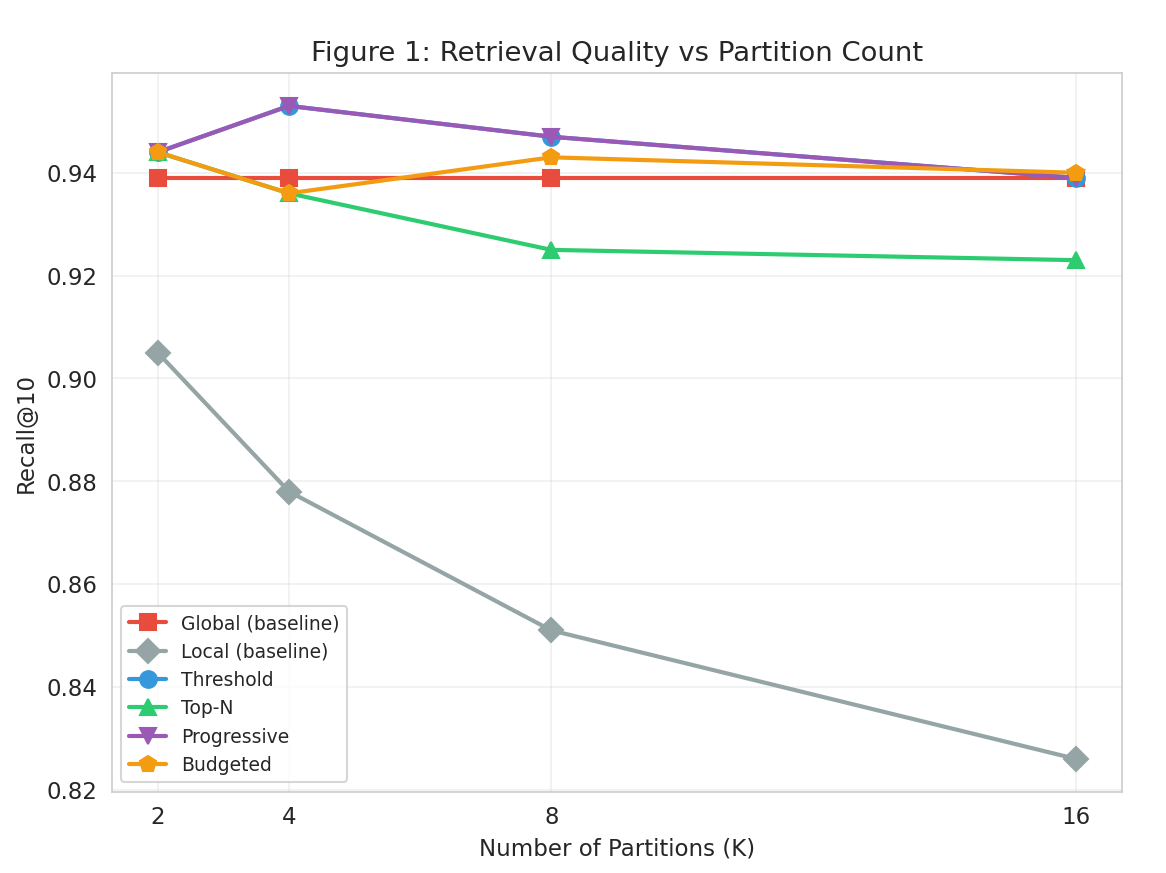
\includegraphics[width=\linewidth]{figure1_retrieval_qualityVsPartitionCount.png}
    \caption{Recall@10 vs Number of Partitions. Adaptive strategies maintain stable recall while local-only degrades.}
    \label{fig:recall}
\end{figure}

\subsection{Communication-Quality Tradeoff}

Figure~\ref{fig:pareto} illustrates the Pareto frontier between communication cost and retrieval quality. Adaptive strategies occupy the efficient frontier, achieving higher recall per unit of communication compared to both global and local baselines.

\begin{figure}[h]
    \centering
    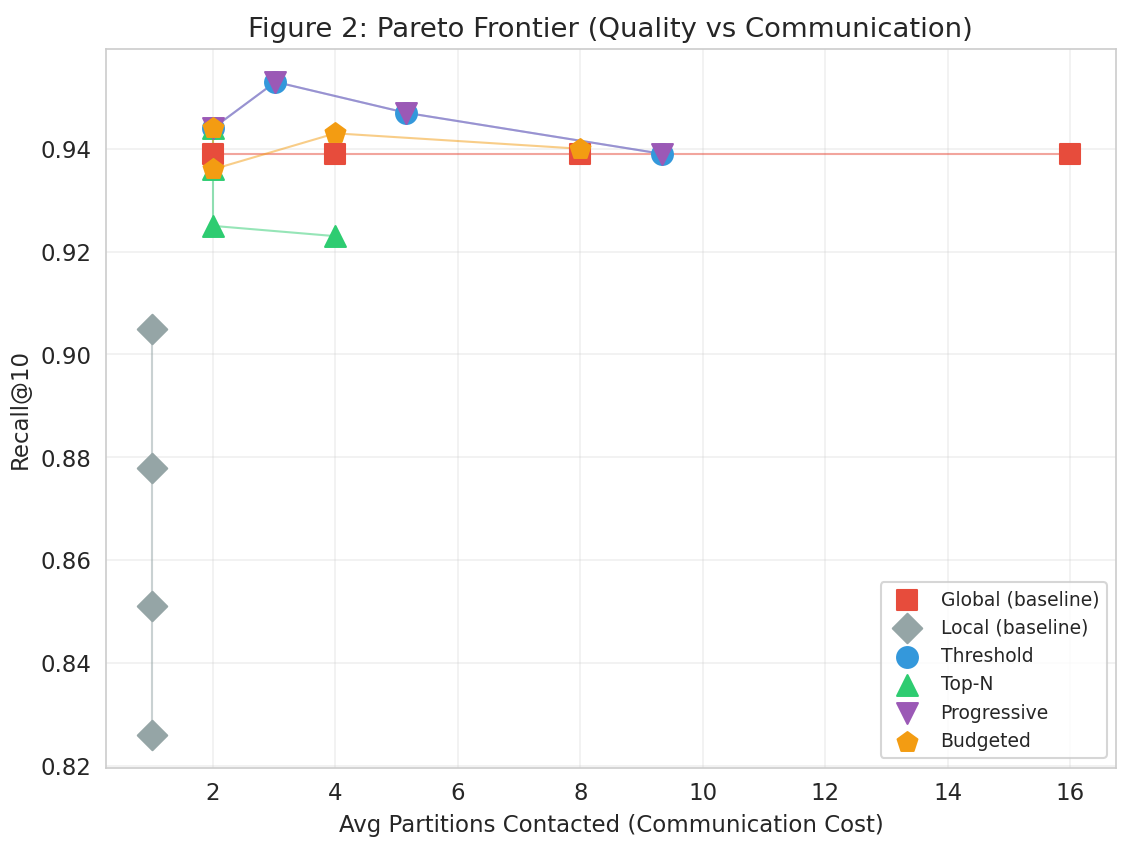
\includegraphics[width=\linewidth]{figure2_pareto_frontier(qualityvsCommunication).png}
    \caption{Pareto frontier: Communication cost vs Recall@10. Adaptive strategies achieve comparable recall with significantly less communication.}
    \label{fig:pareto}
\end{figure}

\section{Discussion}

\subsection{When Does Routing Help Most?}

Routing provides the greatest benefit when:
\begin{itemize}
    \item The number of partitions is large (K $\geq$ 8), enabling significant communication reduction
    \item The semantic space has moderate to high cluster coherence
    \item Query distribution spans multiple semantic domains
\end{itemize}

At K=2, routing provides minimal benefit because both partitions must be contacted anyway. The value of routing increases monotonically with $K$.

\subsection{Cost-Benefit Analysis}

The Threshold strategy at K=16 achieves:
\begin{itemize}
    \item 42\% reduction in communication (9.3 vs 16 partitions)
    \item 100\% retention of global recall (0.939 = 0.939)
    \item Slight latency increase (14.52ms vs 8.54ms) due to sequential partition queries
\end{itemize}

This represents a favorable tradeoff for systems where communication cost dominates latency.

\subsection{Semantic Space Analysis}

Our dataset exhibits low silhouette scores (0.027--0.046), indicating a continuous semantic space without natural cluster boundaries. Despite this, adaptive routing achieves significant communication savings, suggesting that even subtle semantic differences between partitions can be exploited by confidence-based routing.

We hypothesize that datasets with more naturally separated clusters could yield even higher communication savings, as routing would more effectively identify irrelevant partitions. This suggests potential for even greater efficiency gains in domain-specific applications where semantic categories are more distinct.

\subsection{Limitations}

\begin{itemize}
    \item Communication is simulated on a single machine; network latency and partition distribution are not modeled
    \item Embeddings are pre-computed; incremental index updates are not evaluated
    \item The confidence formula uses fixed hyperparameters ($\theta=0.5$, sigmoid slope=5); adaptive tuning may improve performance
    \item Dataset size (100K) is smaller than production-scale systems (millions to billions)
\end{itemize}

\section{Conclusion}

We presented four adaptive routing strategies for distributed vector memory that reduce communication costs while maintaining retrieval quality. Our key findings:

\begin{enumerate}
    \item Adaptive routing matches global recall (0.939) with 42\% less communication at K=16
    \item Budgeted communication can slightly exceed global recall by reducing noise
    \item Semantic partitioning (KMeans) outperforms random partitioning by 8--12\%
    \item The communication savings increase with partition count, suggesting favorable scaling properties
\end{enumerate}

\textbf{Future work:} We plan to investigate hierarchical scaling (distribution of distributions) to achieve sub-linear communication growth, evaluate performance on production-scale datasets with natural semantic clusters, and develop adaptive threshold tuning mechanisms.

\subsection{Connection to Probabilistic Computing}

Our confidence estimation formula is inspired by the eta ratio ($\eta = f_{\text{comm}} / f_{\text{p-bit}}$) from probabilistic computing~\cite{aadit2026programmable}, which quantifies the tradeoff between communication frequency and local computation in partitioned stochastic systems. Aadit et al.~demonstrate that above a topology-dependent threshold, a distributed probabilistic machine matches a monolithic reference, while below it, accuracy degrades as a power law. Our coverage term $\frac{n_{\text{contacted}}}{n_{\text{total}}}$ plays an analogous role: it penalizes low partition contact, preventing premature termination in the same way that insufficient boundary refresh degrades the distributed sampler. This connection suggests that our adaptive routing strategies may generalize beyond vector search to other partitioned stochastic systems.

\bibliographystyle{plain}

\begin{thebibliography}{10}

\bibitem{hnsw}
Yu A. Malkov and D. A. Yashunin.
\newblock Efficient and robust approximate nearest neighbor search using Hierarchical Navigable Small World graphs.
\newblock {\em IEEE Transactions on Pattern Analysis and Machine Intelligence}, 42(4):824--836, 2019.

\bibitem{zhang2015character}
Xiang Zhang, Junbo Zhao, and Yann LeCun.
\newblock Character-level Convolutional Networks for Text Classification.
\newblock In {\em Advances in Neural Information Processing Systems}, volume 28, 2015.

\bibitem{reimers2019sentence}
Nils Reimers and Iryna Gurevych.
\newblock Sentence-BERT: Sentence Embeddings using Siamese BERT-Networks.
\newblock In {\em Proceedings of the 2019 Conference on Empirical Methods in Natural Language Processing}, pages 3982--3992, 2019.

\bibitem{turboquant}
Amir Zandieh, {et al.}
\newblock TurboQuant: Online Vector Quantization with Near-optimal Distortion Rate.
\newblock In {\em International Conference on Learning Representations (ICLR)}, 2026.

\bibitem{fedvs}
Zeheng Fan, Yuxiang Zeng, Zhuanglin Zheng, and Yongxin Tong.
\newblock FedVS: Towards Federated Vector Similarity Search with Filters.
\newblock In {\em Proceedings of the 31st ACM SIGKDD Conference on Knowledge Discovery and Data Mining}, 2025.

\bibitem{dhnsw}
Fei Fang, Yi Liu, and Chen Qian.
\newblock d-HNSW: A High-performance Vector Search Engine on Disaggregated Memory.
\newblock {\em Proceedings of the ACM on Measurement and Analysis of Computing Systems}, 10(2):1--28, 2026.

\bibitem{shardmemo}
Yang Zhao, Chengxiao Dai, Yue Xiu, Mengying Kou, Yuliang Zheng, and Dusit Niyato.
\newblock ShardMemo: Masked MoE Routing for Sharded Agentic LLM Memory.
\newblock {\em arXiv preprint arXiv:2601.21545}, 2026.

\bibitem{hyphaedb}
HyphaeDB Authors.
\newblock HyphaeDB: A Living Knowledge Topology for Agent-First Memory Using HNSW Graph Structure as a Gossip-Based Communication Fabric.
\newblock {\em arXiv preprint}, 2026.

\bibitem{ragroute}
Akash Dhasade, Rachid Guerraoui, Anne-Marie Kermarrec, Diana Petrescu, Rafael Pires, Mathis Randl, and Martijn de Vos.
\newblock Efficient Federated Search for Retrieval-Augmented Generation using Lightweight Routing.
\newblock In {\em Proceedings of the 5th Workshop on Machine Learning and Systems (EuroMLSys)}, 2025.

\bibitem{pyramid}
Shiyuan Deng, Xiao Yan, Kelvin K. W. Ng, Chenyu Jiang, and James Cheng.
\newblock Pyramid: A General Framework for Distributed Similarity Search on Large-scale Datasets.
\newblock In {\em IEEE International Conference on Big Data}, pages 1066--1071, 2019.

\bibitem{aadit2026programmable}
Navid Anjum Aadit, Xiuqi Zhang, Shuvro Chowdhury, Kevin Callahan-Coray, Kyle Lee, Saleh Bunaiyan, Sanjay Seshan, Clayton Thomas, Jason Twigg, Andrew Seawright, Forrest Brewer, Tathagata Srimani, and Kerem Y. Camsari.
\newblock Programmable Probabilistic Computer with 1,000,000 p-bits.
\newblock {\em arXiv preprint arXiv:2606.25313}, 2026.

\end{thebibliography}

\end{document}
